\beginsong{Die Brombeeren}[wuw={Volkslied aus Lothringen, 19. Jahrhundert}, bo={144}, pfii={78}, pfiii={41}, index={Es wollt ein Mägdlein}]

\beginverse
\endverse
\centering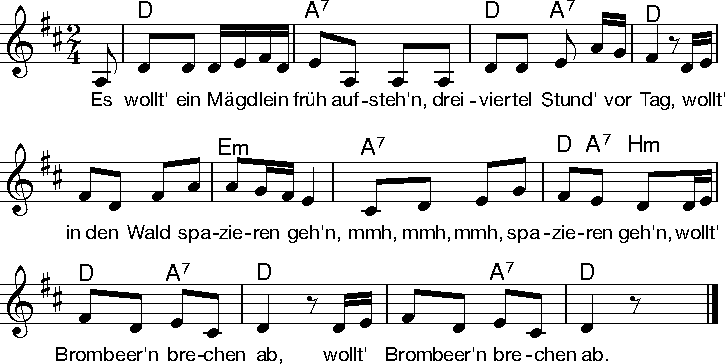
\includegraphics[width=1\textwidth]{Noten/Lied021.pdf}	

\beginverse
Und \[D]als sie in den \[A7]Wald 'nein kam, da \[D]kam des \[A7]Jägers K\[D]necht:
''Ei Mädchen, scher dich \[Em]aus dem Wald! \[A7]Mmmh mmmh \[D]aus \[A7]dem \[Hm]Wald!
\lrep  Meinem \[D]Herr'n, dem \[A7]ist's nicht \[D]recht.'' \rrep
\endverse

\beginverse
Und ^als sie ein Stück ^weiter kam, da ^kam des ^Jägers ^Sohn:
''Ei Mädchen, setz dich ^nieder, ^mmmh mmmh setz dich ^ni^e^der,
\lrep  zupf ^dir dein ^Körblein ^voll!'' \rrep
\endverse

\beginverse
''Ein ^Körblein voll, das b^rauch ich nicht, ein ^Handvoll ^ist ge^nug.
In meines Vaters ^Garten, ^mmmh mmmh ^Ga^r^ten,
\lrep  da ^wachsen ^Brombeeren ^genug.' \rrep
\endverse

\beginverse
So ^schön wie braune ^Bären sah ^sie seine ^Äuglein ^steh'n.
Wer kann im grünen ^Walde, ^mmmh mmmh im grünen ^Wa^l^de,
\lrep den ^Beeren ^wider^steh'n? \rrep
\endverse

\beginverse
Und ^als dreiviertel Jahr ver^gangen war'n, die ^Brombeeren ^wurden ^groß,
da hat das schwarzbraun ^Mägdelein, ^mmmh mmmh das ^Mäg^de^lein,
\lrep ein ^Kind auf ^ihrem ^Schoß. \rrep
\endverse

\beginverse
Sie ^schaut es mit Ver^wund'rung an: 'Ei ^ei, was ^hab' ich denn ge^tan?
Kommt das wohl von den ^Brombeeren, ^mmmh mmmh, von den ^Brom^bee^ren,
\lrep die ^ich ge^pflücket ^hab'?' \rrep
\endverse

\beginverse
D'rum ^wer ein ehrliches ^Mägdlein will ham, der ^schick sie nicht ^in den ^Wald,
denn im Wald da wachsen ^Brombeeren, ^ja, ja, ja, die ^Brom^bee^ren,
\lrep und die ^reifen manchmal ^viel zu ^bald. \rrep
\endverse


\endsong
